\chapter[Referencial Teórico]{Referencial Teórico}

Este capítulo apresenta a teoria estudada para a implementação dos objetivos deste trabalho. Primeiramente, discute os princípios do aprendizado de máquina, aprendizado profundo, redes neurais artificiais e aprendizado por reforço. Por fim, aborda os desafios e trabalhos relacionados em modelos baseados em aprendizado nas competições de futebol de robôs.

\section{Inteligência Artificial}

\subsection{Aprendizado de Máquina e Aprendizado Profundo}

O aprendizado de máquina é um subcampo da inteligência artificial que busca desenvolver algoritmos capazes de aprender padrões a partir de dados, sem serem explicitamente programados \cite{goodfellow2016deep}. Dentro desse campo, o Aprendizado Profundo se destaca por utilizar redes neurais com múltiplas camadas para aprender representações hierárquicas e abstratas dos dados, sendo especialmente eficaz em tarefas complexas, como reconhecimento de padrões e previsão de comportamentos \cite{lecun2015deep}.


\subsection{Redes Neurais Artificiais}

Redes Neurais Artificiais (RNAs) são modelos computacionais inspirados no funcionamento do cérebro humano, compostos por neurônios interconectados organizados em camadas \cite{haykin2007redes}. Cada neurônio recebe entradas, processa-as por meio de uma função de ativação e gera uma saída que é propagada para neurônios subsequentes. A estrutura básica de uma RNA inclui:

\begin{itemize}
    \item \textbf{Camada de Entrada}: Responsável por receber os dados brutos do problema. Cada neurônio nesta camada representa uma variável de entrada do modelo, denotada por $x_i$, onde $i = 1, 2, ..., n$. A quantidade de neurônios nesta camada é determinada pela dimensionalidade dos dados de entrada.
    
    \item \textbf{Camadas Ocultas}: Realizam transformações não lineares nos dados, extraindo características relevantes. Cada neurônio recebe um conjunto de entradas ponderadas pelos pesos sinápticos $w_{ij}$ e aplica uma função de ativação para gerar uma saída. O número de camadas ocultas e a quantidade de neurônios em cada uma influenciam a capacidade de aprendizado da rede.
    
    \item \textbf{Camada de Saída}: Produz a predição final do modelo. A quantidade de neurônios nesta camada depende do tipo de problema: para classificação binária, geralmente há um único neurônio com função de ativação sigmoide; para classificação multiclasse, usa-se a função \textit{softmax} com tantos neurônios quanto categorias; para problemas de regressão, a saída pode ser um único valor real sem ativação ou com uma ativação linear.
\end{itemize}

A escolha da função de ativação é crucial para o desempenho da rede. Funções como \textit{ReLU} (Rectified Linear Unit) e \textit{sigmoide} são comumente utilizadas para introduzir não-linearidades e permitir que a rede aprenda padrões complexos \cite{goodfellow2016deep}. A Figura~\ref{fig:rede_neural} ilustra a estrutura básica de um neurônio artificial. 

\begin{figure}[!htpb]
\centering
\caption{Esquema de um neurônio artificial, onde $x_i$ representa as entradas, $w_i$ os pesos sinápticos, $\sum$ a soma ponderada, $f$ a função de ativação e $y$ a saída.}

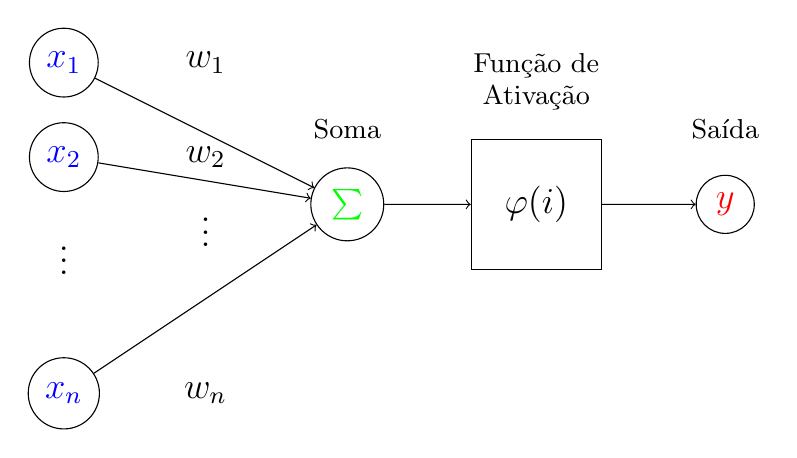
\begin{tikzpicture}[scale=1.2, every node/.style={scale=1.1}]

    % Nós das entradas
    \node[draw, circle] (x1) at (0,2) {\large \textcolor{blue}{$x_1$}};
    \node[draw, circle] (x2) at (0,1) {\large \textcolor{blue}{$x_2$}};
    \node (xdots) at (0,0) {\large $\vdots$};
    \node[draw, circle] (xn) at (0,-1.5) {\large \textcolor{blue}{$x_n$}};
    % Pesos
    \node (w1) at (1.5,2) {\large $w_1$};
    \node (w2) at (1.5,1) {\large $w_2$};
    \node (wdots) at (1.5,0.3) {\large $\vdots$};  % Movido um pouco para cima
    \node (wn) at (1.5,-1.5) {\large $w_n$};

    % Soma
    \node[draw, circle] (sum) at (3,0.5) {\large \textcolor{green}{$\sum$}};
    
    % Texto acima da soma
    \node at (3,1.3) {\small \shortstack{Soma}};

    % Função de ativação
    \node[draw, rectangle, minimum width=1.5cm, minimum height=1.5cm] (activation) at (5,0.5) {\large $\varphi(i)$};
    
    % Texto acima da função de ativação
    \node at (5,1.8) {\small \shortstack{Função de \\ Ativação}};
    % Saída
    \node[draw, circle] (output) at (7,0.5) {\large \textcolor{red}{$y$}};
    
    % Texto acima da saída
    \node at (7,1.3) {\small \shortstack{Saída}};
    
    % Conexões das entradas à soma
    \draw[->] (x1) -- (sum);
    \draw[->] (x2) -- (sum);
    \draw[->] (xn) -- (sum);

    % Conexões da soma à função de ativação
    \draw[->] (sum) -- (activation);

    % Conexão da função de ativação à saída
    \draw[->] (activation) -- (output);

\end{tikzpicture}
\fonte{Autor}
\label{fig:rede_neural}
\end{figure}


\subsection{\textit{Long Short Term Memory}}  

As Redes Neurais Recorrentes (RNNs) são arquiteturas projetadas para processar dados sequenciais, porém enfrentam limitações como o desaparecimento do gradiente, que restringe o aprendizado de dependências de longo prazo \cite{hochreiter1997long}. Para contornar esse problema, as redes LSTM (Long Short-Term Memory) foram desenvolvidas com células de memória e portas lógicas que regulam dinamicamente o fluxo de informações\ a Figura \ref{fig:LSTM} mostra um exemplo de arquitetura desse tipo. Essa arquitetura permite que LSTMs capturem relações temporais complexas em séries de dados, superando RNNs tradicionais em tarefas como previsão de trajetórias e modelagem de sistemas não lineares \cite{gers2000learning}. Estudos comparativos destacam sua eficácia em cenários onde modelos físicos são desconhecidos ou incompletos, como na filtragem adaptativa de sinais ruidosos \cite{greff2017lstm}.

\begin{figure}
    \centering
    \caption{Exemplo de Arquitetura de uma LSTM}
    \includegraphics[width=0.7\linewidth]{figuras/LSTM.png}
    \fonte{\cite{sak2014long}}
    \label{fig:LSTM}
\end{figure}

\subsection{Aprendizado por Reforço}

O Aprendizado por Reforço (RL) é uma abordagem de aprendizado de máquina na qual um agente aprende a tomar decisões através de interações com o ambiente, buscando maximizar uma recompensa cumulativa \cite{Sutton2018}. No contexto da robótica multiagente, o RL tem sido aplicado para treinar agentes a cooperar e competir em ambientes complexos, como no futebol de robôs \cite{Stone2005}. O processo de RL é dividido em 4 partes principais:

\begin{itemize}
    \item \textbf{Agente}: Entidade que toma decisões.
    \item \textbf{Ambiente}: Contexto no qual o agente opera.
    \item \textbf{Ações}: Comportamentos que o agente pode executar.
    \item \textbf{Recompensas}: Feedback numérico que guia o aprendizado.
\end{itemize}

O agente aprende uma política ótima que mapeia estados do ambiente para ações, maximizando a recompensa ao longo do tempo. Técnicas como \textit{Q-learning} e \textit{Deep Q-Networks} (DQNs) têm sido utilizadas para resolver problemas complexos de controle e navegação em robótica \cite{Kober2013}. No entanto, a velocidade de convergência desses métodos representa um desafio significativo, especialmente em ambientes adversários, como no domínio do \textit{RoboCup Soccer}. Se a taxa de aprendizado do agente for muito baixa, o algoritmo pode exigir muitas iterações para aprender a tarefa de forma eficiente, o que pode resultar em derrotas antes que o agente atinja uma política ótima. Para superar esse problema, técnicas como estimativas parciais do estado podem ser empregadas quando parte da dinâmica do ambiente é conhecida ou fácil de modelar, acelerando a convergência do \textit{Q-learning} \cite{Ahumada2013}.

\subsection{\textit{Deep Q-Networks} (DQN)}

O DQN é uma extensão do \textit{Q-learning} que utiliza uma rede neural para aproximar a função de valor Q. A função Q é definida como:

\[
Q(s, a) = \mathbb{E}\left[ R_t + \gamma \max_{a'} Q(s', a') \mid s, a \right]
\]

onde:
\begin{itemize}
    \item \( s \) é o estado atual.
    \item \( a \) é a ação tomada.
    \item \( R_t \) é a recompensa imediata.
    \item \( \gamma \) é o fator de desconto (entre 0 e 1).
    \item \( s' \) é o próximo estado.
    \item \( a' \) é a próxima ação.
\end{itemize}

A rede neural é treinada para minimizar a função de perda:

\[
L(\theta) = \mathbb{E}\left[ \left( R_t + \gamma \max_{a'} Q(s', a'; \theta^-) - Q(s, a; \theta) \right)^2 \right]
\]

onde:
\begin{itemize}
    \item \( \theta \) são os parâmetros da rede neural.
    \item \( \theta^- \) são os parâmetros de uma rede alvo (\textit{target network}), que é atualizada periodicamente para estabilizar o treinamento.
\end{itemize}

\subsection{\textit{Policy Gradient}}

O método \textit{Policy Gradient} busca otimizar diretamente a política \( \pi(a|s; \theta) \), que é uma distribuição de probabilidade sobre as ações dado um estado. A função objetivo é maximizar a recompensa esperada:

\[
J(\theta) = \mathbb{E}_{\tau \sim \pi_\theta} \left[ \sum_{t=0}^T \gamma^t R_t \right]
\]

onde \( \tau \) é uma trajetória gerada pela política \( \pi_\theta \). O gradiente da função objetivo é dado por:

\[
\nabla_\theta J(\theta) = \mathbb{E}_{\tau \sim \pi_\theta} \left[ \sum_{t=0}^T \nabla_\theta \log \pi(a_t|s_t; \theta) \, G_t \right]
\]

onde \( G_t = \sum_{k=t}^T \gamma^{k-t} R_k \) é o retorno descontado a partir do tempo \( t \).



% \section{Filtro de Kalman Estendido (EKF)}  


% O Filtro de Kalman Estendido (EKF) é uma generalização do Filtro de Kalman clássico\cite{Kalman1960} para sistemas não lineares, essencial para estimar estados dinâmicos em robótica quando modelos de movimento ou observação são não lineares\cite{ribeiro2004kalman}. O EKF irá filtrar ruídos nos logs de posição dos robôs, gerando trajetórias mais precisas para treinar as redes neurais e fazer tratamento de dados para preenchimento de lacunas temporais.
  


\section{A Competição \textit{Small Size League} (SSL)}

A \textit{Small Size League (SSL)} é uma das categorias da \textit{RoboCup}, uma competição internacional que visa promover avanços em robótica e inteligência artificial através de desafios práticos e competitivos \cite{kitano1997robocup}. Na SSL, dois times, compostos por 6 ou 11 robôs autônomos, competem em partidas que simulam jogos de futebol. A principal característica dessa categoria é a autonomia dos robôs, que são controlados remotamente por um computador central, responsável por processar informações do ambiente e enviar comandos para a execução de estratégias predeterminadas \cite{zickler2009shared}.

O ambiente de jogo é monitorado por um sistema de câmeras posicionadas acima do campo, que capturam imagens em tempo real. Essas imagens são processadas por um sistema de visão computacional unificado, que identifica a posição dos robôs, da bola e de outros elementos relevantes. Com base nessas informações, o sistema central calcula as ações ideais para cada robô, permitindo que eles se movimentem e interajam de forma autônoma no campo \cite{rocha2012ssl}.

Os robôs utilizados na competição SSL são equipados com rodas omnidirecionais, essa configuração permite realizar movimentos em qualquer direção sem a necessidade de reorientação \cite{romero2014robotica}. O controle do movimento é feito ajustando as velocidades de cada roda, o que possibilita alterar a velocidade linear, angular e a orientação do robô no campo.

A competição destaca-se pelo uso de tecnologias avançadas em robótica, sistemas embarcados e visão computacional, proporcionando um ambiente propício para o desenvolvimento e aplicação de técnicas de controle e inteligência artificial \cite{stone2000layered}.

\subsection{Dimensões do Campo}

O campo utilizado na Divisão B da SSL possui dimensões padronizadas de 10,4 metros de comprimento por 7,4 metros de largura, com uma área de jogo efetiva de 9 metros por 6 metros. As marcações do campo, como as linhas de fundo, laterais, áreas do gol e círculo central, seguem padrões definidos pela organização da competição. Pequenas variações nas dimensões lineares (até ±10\%) são permitidas para acomodar diferentes configurações de arena \cite{robocup2023rules}.

A Figura \ref{fig:dimensoes_campo } ilustra as dimensões e marcações do campo da Divisão B, conforme estabelecido pelas regras oficiais da RoboCup\cite{robocup2023rules}.

\begin{figure}[!htpb]
\centering
\caption{Dimensões do Campo da Divisão B da SSL.}
\includegraphics[width=0.9\linewidth]{figuras/dimensões_campo.png}
\fonte{\cite{robocup2023rules}}
\label{fig:dimensoes_campo }
\end{figure}

\subsection{Sistema de Visão e Identificação dos Robôs}

O sistema de visão utilizado na SSL é unificado e padronizado para todas as equipes, garantindo compatibilidade e justiça competitiva \cite{zickler2009shared}. Esse sistema é composto por câmeras de alta resolução posicionadas acima do campo, que capturam imagens em tempo real. As imagens são processadas por algoritmos de visão computacional para identificar a posição dos robôs, da bola e de outros elementos relevantes.

Cada robô é equipado com marcadores visuais padronizados, que permitem sua identificação única durante as partidas. Esses marcadores consistem em padrões de cores específicos, conforme ilustrado na Figura \ref{fig:cores_robos}. A diferenciação entre os times é feita pela cor central do marcador, que pode ser azul ou amarela. As equipes devem concordar previamente sobre a escolha das cores, não sendo permitido que ambos os times utilizem a mesma cor central \cite{robocup2023rules}.

\begin{figure}
    \centering]
    \caption{Marcadores Visuais dos Robôs}
    \includegraphics[width=0.5\linewidth]{figuras/cores_robos.png}
    \fonte{\cite{robocup2023rules}}
    \label{fig:cores_robos}
\end{figure}


\subsection{\textit{Game Controller}}  
O \textit{Game Controller} da RoboCup Small Size League (SSL) é um sistema automatizado que atua como árbitro central, gerenciando o fluxo do jogo e garantindo conformidade com as regras. Ele controla estados do jogo (e.g., kickoff, penalty), inicia/pausa partidas, define o placar e aplica penalidades por infrações (e.g., invasão de área), comunicando-se com as equipes via protocolo de rede UDP. Sua função é padronizar a execução da partida, substituindo a intervenção humana e permitindo que os robôs operem de forma totalmente autônoma.  

Integrado ao sistema SSL-Vision (que rastreia posições de robôs e bola), o Game Controller fornece dados em tempo real para as equipes, que devem interpretar seus comandos para ajustar estratégias dinâmicas. Essa integração é essencial para manter a justiça e a sincronia em ambientes competitivos, onde decisões milissegundos e precisão são críticas.  


% \subsection{Resumo do Jogo}

% Uma partida da categoria B da SSL tem a seguinte duração:

% \begin{table}[h!]
% \centering
% \begin{tabular}{|c|c|}
% \hline
% \textbf{Tempo}      & \textbf{Duração}     \\ \hline
% Primeiro Tempo      & 6 minutos            \\ \hline
% Intervalo           & 3 minutos            \\ \hline
% Segundo Tempo       & 6 minutos            \\ \hline
% \end{tabular}
% \caption{Duração de uma partida na categoria B da SSL.}
% \end{table}



\subsection{Estados do Jogo e Regras}

Os estados do jogo são controlados pelo \textit{Game Controller} e indicam as fases operacionais da partida. Abaixo estão os principais estados do jogo:

\begin{table}[h!]
\centering
\begin{tabular}{c|c}
\hline
\textbf{Estado}      & \textbf{Descrição}                              \\ \hline
\textbf{Halt}         & Jogo parado (início ou após infrações graves).  \\ 
\textbf{Stop}         & Jogo pausado (ex.: bola saiu do campo).         \\ 
\textbf{Running}      & Jogo em andamento, com robôs operando livremente. \\ 
\textbf{Kickoff}      & Reinício no centro do campo após gol ou início de período. \\ 
\textbf{Free Kick}    & Cobrança de falta (defensores a 0.5 m da bola). \\ 
\textbf{Penalty Kick} & Cobrança de pênalti (apenas cobrador e goleiro na área). \\ 
\textbf{Timeout}      & Pausa solicitada por uma equipe (limitado a 2 por partida). \\ \hline
\end{tabular}
\caption{Estados do jogo na SSL RoboCup.}
\end{table}

\subsection{Resumo das Regras}  
Cada equipe pode ter até 6 robôs, obedecendo às dimensões máximas de 22 cm de altura e 18 cm, a Figura \ref{fig:alvim} mostra um exemplo de uma categoria de entrada, a SSL-EL da Robocup Brasil desenvolvido pela equipe da Universidade de Brasília Titans. 


\begin{figure}[!htpb]
    \centering
    \caption{Robô da liga SSL-EL desenvolvido pela Titans - UnB}
    \includegraphics[width=0.5\linewidth]{figuras/alvim_ssl.png}
    \fonte{Autor}
    \label{fig:alvim}
\end{figure}


A bola deve permanecer em movimento contínuo, e tocar robôs parados resulta em falta. Um gol é validado apenas quando a bola ultrapassa completamente a linha do gol, incluindo situações de chutes diretos ou deflexões.  As infrações são categorizadas como colisões violentas (punidas com cartão amarelo ou vermelho), toque manual (que paralisa o jogo imediatamente) ou posicionamento ilegal (com remoção temporária do robô). A partida é dividida em dois períodos de 6 minutos, com intervalo de 3 minutos, e substituições são permitidas apenas durante os estados \textit{Stop} ou \textit{Halt}, realizadas fora da área técnica para evitar interferência no jogo.  


% \section{Trabalhos Relacionados}

% Diversos trabalhos têm explorado o uso de deep learning e RL para prever comportamentos em robótica. Por exemplo, \cite{Kahn2018} utilizou CNNs para analisar trajetórias de robôs, enquanto \cite{Riedmiller2009} aplicou RL para prever movimentos de adversários no futebol de robôs. Essas abordagens demonstram o potencial das técnicas de aprendizado de máquina para melhorar a autonomia e a eficiência de sistemas robóticos.